\chapter{實驗結果} \label{se_6}
本章節對我們實作的TwoStepBFT進行測試。測試的節點皆是在Amazon EC2 t2.small上運行。t2.small 的硬體規格為1個虛擬CPU 與2GB 的記憶體。交易型態則是基本的以太坊轉帳交易。我們以交易的吞吐量Throughput(每秒共識多少筆交易量)與區塊的延遲性latency(完成一個區塊共識平均需要多少時間)來衡量共識的效率。我們也測試共識演算法的延展性(Scalability),以瞭解當參與共識的節點數量變多時,共識效能會受到怎樣的影響。最後,我們將節點分散部署在世界各地,讓該系統較貼近真實的應用場景並且與同資料中心實驗比較。
\section{環境建設}\label{se_6}
利用第五章所述方法部署私有鏈後,我們先讓節點互相交易約15分鐘,讓交易存入交易池內,這可以讓共識時產生的區塊塞滿足夠的交易。接下來將運行共識演算法約一小時,並將結果紀錄下來。
\section{同資料中心吞吐量與延遲性測試}\label{se_6}
此小節我們將探討我們的演算法在同資料中心的實驗環境下,觀察吐量與延遲性的變化。我們將機器都運行於美國-奧勒岡資料中心。
對於測試基本的交易吞吐量與延遲性測試,我們透過控制創世區塊裡的GasLimit來控制單個區塊能包含的最大交易數量,區塊大小分別為每個區塊包含500、1000、4000、8000筆交易。實驗總共進行了五種節點數分別是16、30、60、80、100 個節點。
\begin{figure}[htp]
\centering
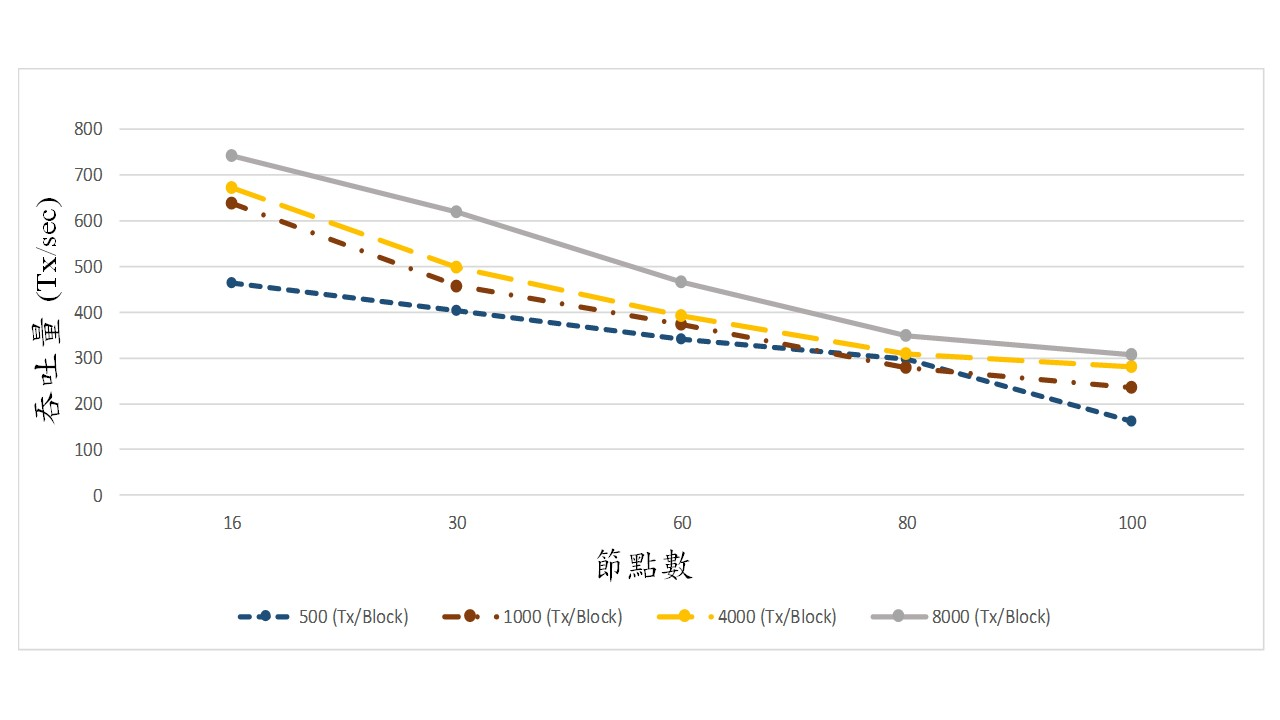
\includegraphics[scale=0.55]{images/61.png}
\caption{吞吐量 V.S 節點數}
\label{i:byz-latency}
\end{figure}
 
%\newpage
\begin{figure}[h]
\centering
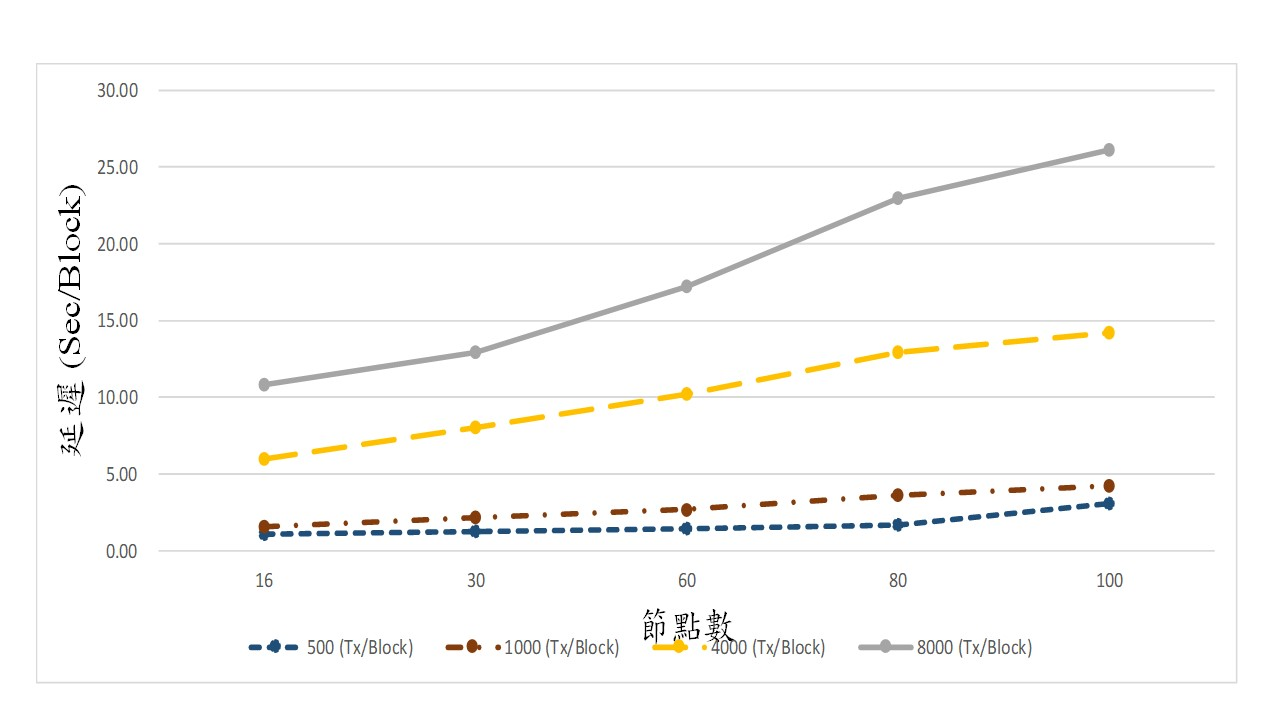
\includegraphics[scale=0.50]{images/62.jpg}
\caption{同資料中心的延遲性表現。}
\label{i:byz-latency}
\end{figure}


從圖6.1中可以看到我們的共識演算法在節點數增加時,吞吐量會隨之降低;而圖6.2則可以看到我們的共識演算法在節點數增加時延遲也會隨之增加,
從圖6.1與圖6.2都能觀察出共識效率隨區塊變大而增加。在100個節點參與共識時,吞吐量依舊能達到每秒300筆交易左右的共識速度,對於節點數的容忍能具有良好的延展性。



\section{誇資料中心吞吐量與延遲性測試}\label{se_6}
此小節我們將探討我們的演算法在跨資料中心的實驗環境下,觀察吐量與延遲性的變化,並與同資料中心實驗進行比較。
與同資料中心的吞吐量與延遲性測試實驗一樣,我們先讓節點互相交易約15分鐘,讓交易存入交易池內。接下來將運行共識演算法約一小時,並將結果紀錄下來。區塊大小分別為每個區塊包含500、1000、4000、8000筆交易。實驗總共進行了五種節點數分別是16、30、60、80、100 個節點。不同的是我們將節點分散的部署在世界各地,這讓實驗更加貼近真實應用。在實驗裡我們將節點平均分散在(美國-奧勒岡、美國-維吉尼亞北部、日本-東京、新加玻、倫敦)。
\begin{figure}[htp]
\centering
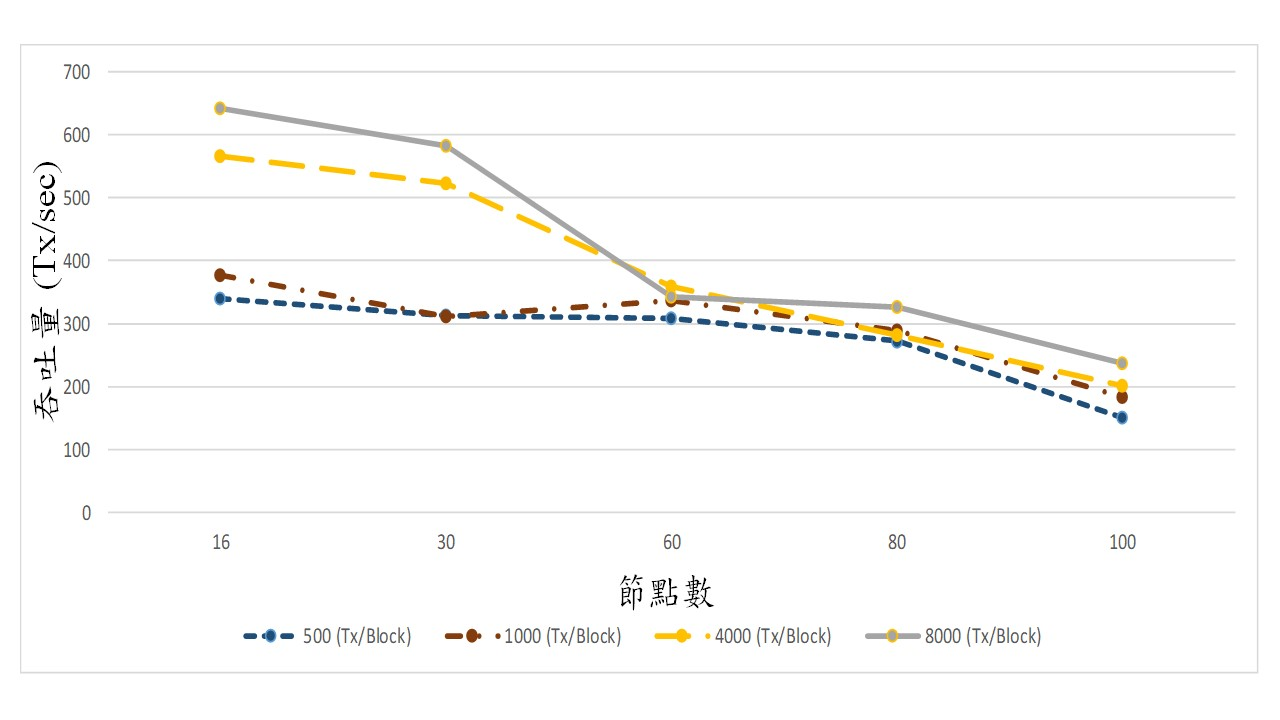
\includegraphics[scale=0.5]{images/63.jpg}
\caption{跨資料中心的交易吞吐量表現。}
\label{i:byz-latency}
\end{figure}

\begin{figure}[htp]
\centering
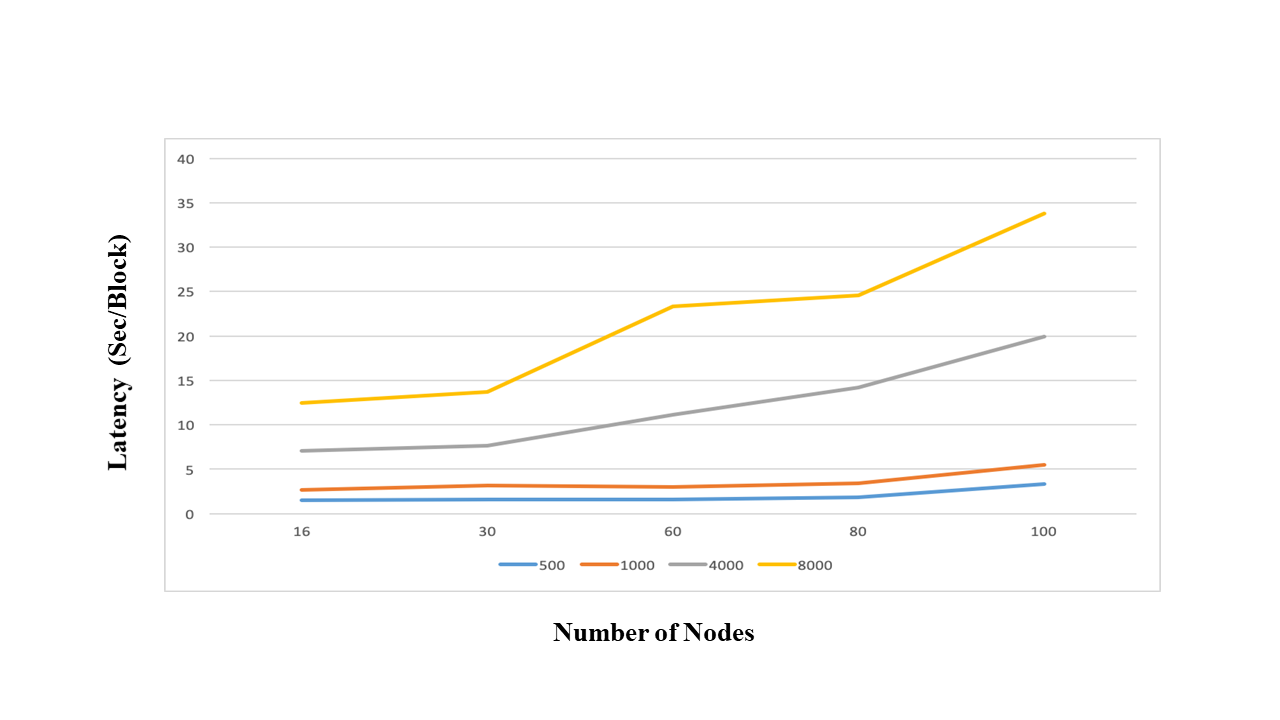
\includegraphics[scale=0.5]{images/64.jpg}
\caption{跨資料中心的延遲性表現。}
\label{i:byz-latency}
\end{figure}


\newpage
從圖6.3中可以看出在跨資料中心實驗裡隨節點數增加時,吞吐量隨之降低。500(Tx/Block)與1000(Tx/Block)吞吐量變化雖然平緩,但從圖6.4能看出延遲也沒有大幅上升;相比之下 4000(Tx/Block)與8000(Tx/Block)雖然在16與30個節點時吞吐量較高,但節點數多時延遲卻是大幅增加。實驗顯示即使在跨資料中心實驗裡,100個節點的共識吞吐量依舊能有約300TPS左右。


\begin{figure}[htp]
\centering
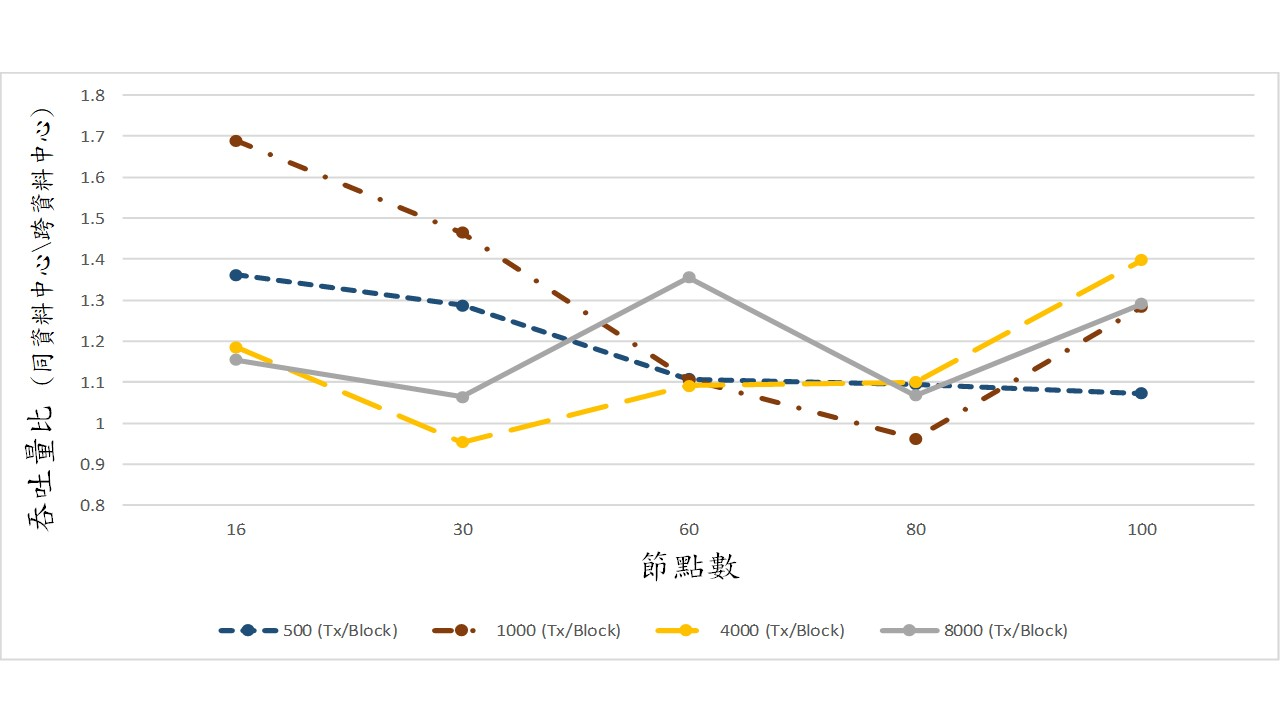
\includegraphics[scale=0.5]{images/65.jpg}
\caption{同資料中心與跨資料中心吞吐量比。}
\label{i:byz-latency}
\end{figure}

\begin{figure}[h]
\centering
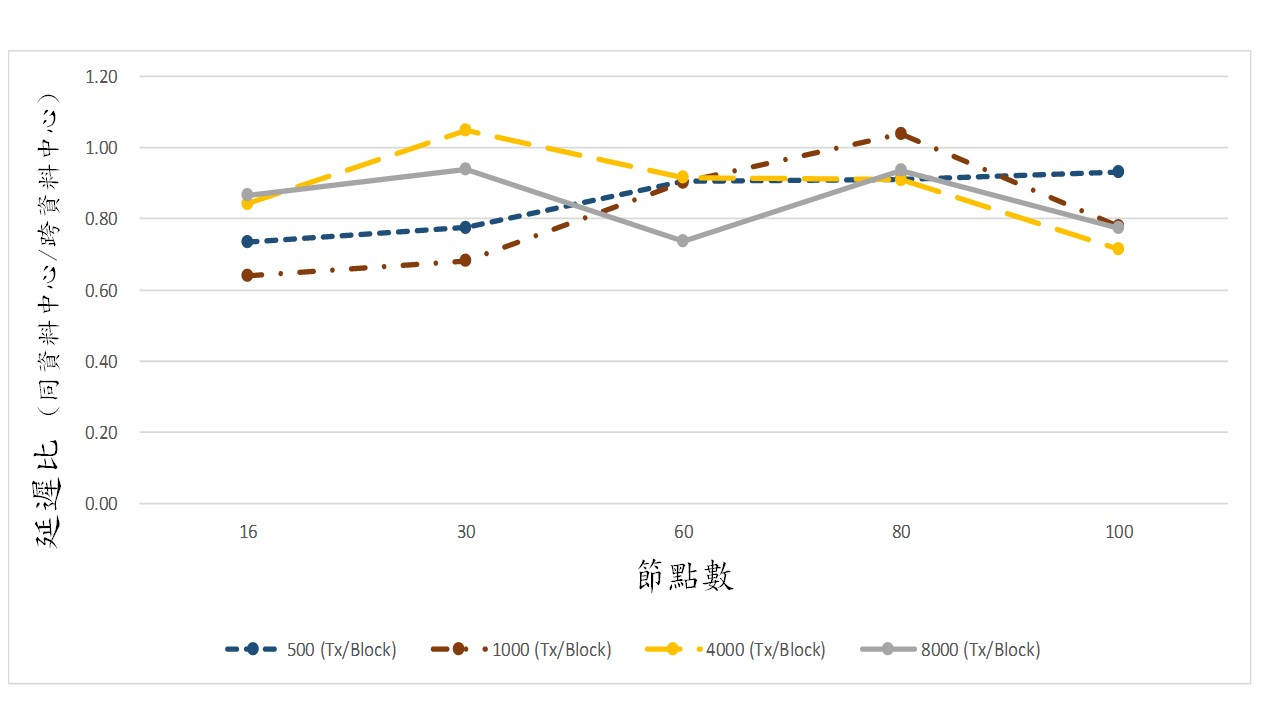
\includegraphics[scale=0.8]{images/66.jpg}
\caption{同資料中心與跨資料中心延遲比。}
\label{i:byz-latency}
\end{figure}

\newpage
圖6.5與圖6.6將同資料中心實驗與跨資料中心實驗作比較,從圖6.5中能觀察到在跨資料中心的實驗裡,吞吐量幾乎皆小於同資料中心的實驗;從圖6.6也可得知跨資料中心實驗延遲也較同資料中心實驗延遲高。從實驗中能觀察到資料中心的設置的確會影響共識效率。



